\clearpage
\chapter{Introduction}
WebRTC is short for web real-time communication, it is an API that modern browser support and can be used by web developers to implement a peer to peer communication. It can be used to capture and stream audio and/or video data, as well as to exchange arbitrary data between browser without requiring an intermediary.

\section{Support}
All major browser support WebRTC in its newest release. Older versions might not, or only partially, implement this API so the Adapter.js~\autocite{adapterjs} project should be considered for productive solutions. For detailed information on supported browsers use caniuse~\autocite{caniuse}.

\section{Session Establishment}
The session establishment uses different network methods to create connection to a peer. This also includes substitutions for situations where the default connection can not be established.

\begin{figure}[H]
	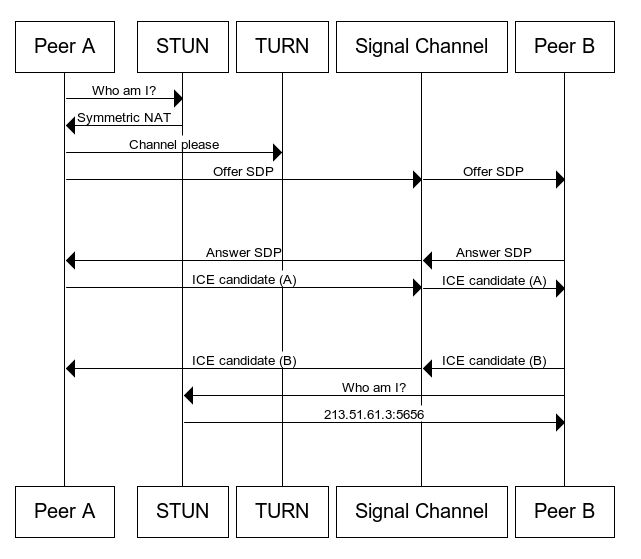
\includegraphics[scale=0.5]{webrtc-complete-diagram.png}
	\centering
	\caption{WebRTC Complete communication schema, \url{https://developer.mozilla.org/en-US/docs/Web/API/WebRTC_API/Connectivity}}
	\label{fig:WebRTC}
\end{figure}

\subsection{Network Address Translation (NAT)}
Is used to give devices in a network a public IP address. This is achieved by translating requests from the device's private IP to the router's public IP with a unique port. The goal is to not need a unique public IP for each device.

\subsection{Session Traversal Utilities for NAT (STUN)}
This protocol is used to discover the public address of the peer. It also will determine any restrictions that would prevent a direct connection with a peer.

The peer sends a 'who am i' request to a STUN server which responds with the public address of the peer.

\begin{figure}[H]
	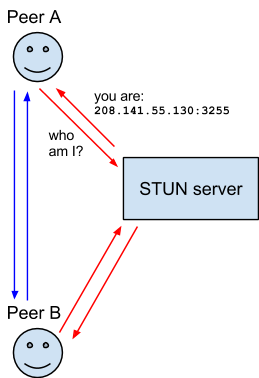
\includegraphics[scale=0.5]{webrtc-stun.png}
	\centering
	\caption{STUN communication schema, \url{https://developer.mozilla.org/en-US/docs/Web/API/WebRTC_API/Protocols}}
	\label{fig:STUN}
\end{figure}

There are some open STUN servers available:
\begin{itemize}
	\item stun.l.google.com:19302
	\item stun[1-4].l.google.com:19302
	\item stunserver.org
	\item stun.schlund.de
	\item stun.voipstunt.com
\end{itemize}

There can be found more online.

\subsection{Traversal Using Relays around NAT (TURN)}
If STUN can't be used, because for example 'Symmetric NAT' is employed in the network, TURN will be used as fallback. This is achieved by opening a connection with a TURN server, this server then will relaying all information through that server.

\begin{figure}[H]
	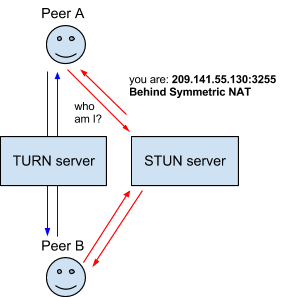
\includegraphics[scale=0.5]{webrtc-turn.png}
	\centering
	\caption{TURN communication schema, \url{https://developer.mozilla.org/en-US/docs/Web/API/WebRTC_API/Protocols}}
	\label{fig:TURN}
\end{figure}

There are open TURN servers, for example provided by google. But this will mean all communication is going threw a foreign server which might not be acceptable.

\subsection{Session Description Protocol (SDP)}
This standard describes the multimedia content of a connection. This includes a resolution, formats, codecs, encryption, etc. basically it is the metadata describing the content not the content itself.

\subsection{ICE Candidates}
Peers have to exchange information about the network connection, this is known as an ICE candidate. Each peer proposes its best candidate, and will work down to the worst candidate until they agree on a common candidate. This wil, be UDP ideally but can be TCP as well.

\section{Security}
Generally WebRTC traffic is encrypted using DTLS. Traffic that is relayed over a TURN server is not necessarily end-to-end encrypted.

\textit{Confidentiality for the application data relayed by TURN is best provided by the application protocol itself, since running TURN over TLS does not protect application data between the server and the peer. If confidentiality of application data is important, then the application should encrypt or otherwise protect its data. For example, for real-time media, confidentiality can be provided by using SRTP.}~\cite{TURN:sec}

\section{Related topics}
There are multiple related topics to WebRTC. In this section we'll try to give a quick overview over the most important ones.

\subsubsection{Media Capture and Streams API}
This API is heavily related to WebRTC, it provides support for streaming audio and video data. Provided are interfaces and methods for working with the success and error callbacks when using the data asynchronously and the events that are fired during the process, as well as the constraints associated with data formats.

\subsection{Web media technologies}
This topic represents all available API's for creating, presenting and managing audio, video and other media. Contained are HTML elements, DOM interfaces and other features.